% ----------------------------------------------------------------------------------------\
% ---------------------------------------------------------------------------------------\
% --------------------------------------------------------------------------------------\
\section{Resultados obtenidos}
% ----------------------------------------------------------------------------------------\
% ---------------------------------------------------------------------------------------\
% --------------------------------------------------------------------------------------\
% Mostrar ejecuciones del código con capturas 
% Mostrar una comparación del código

% ----------------------------------------------------------------------------------------\
% ---------------------------------------------------------------------------------------\
\subsection{Juego de la Vida sin algoritmo genético}
% ----------------------------------------------------------------------------------------\
% ---------------------------------------------------------------------------------------\

A continuación se presentan dos casos diferentes de estados iniciales y se visualiza su 
evolución a través de 5 turnos.

\begin{itemize}
    \item Estado inicial aleatorio\\

\begin{lstlisting}
# Numero de iteraciones/turnos para visualizar
num_iteraciones = 5
n = 10  # Tamano de la matriz

# Generar el estado inicial del juego
estado_actual = crear_matriz_inicial(n)

# Visualizar el estado inicial
visualizar_estado(estado_actual, "Estado Inicial")

# Bucle para actualizar y visualizar el juego en cada turno
for i in range(num_iteraciones):
    # Aplicar las reglas del Juego de la Vida para obtener el nuevo estado
    estado_actual = aplicar_reglas(estado_actual)
    # Visualizar el estado actual despues de aplicar las reglas
    visualizar_estado(estado_actual, titulo=f"Estado despues de {i + 1} turno(s)")
\end{lstlisting}

Los estados se muestran de la siguiente forma:
    \begin{center}
        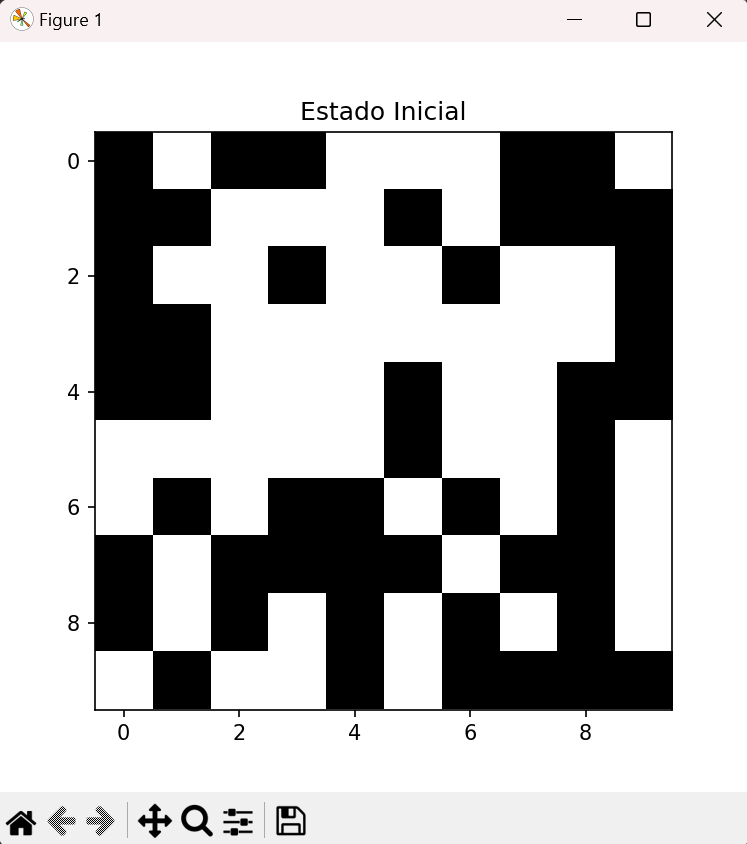
\includegraphics[scale=0.4]{IMA/ejemplosJuegoVida/ejemplo 1.1.png}
        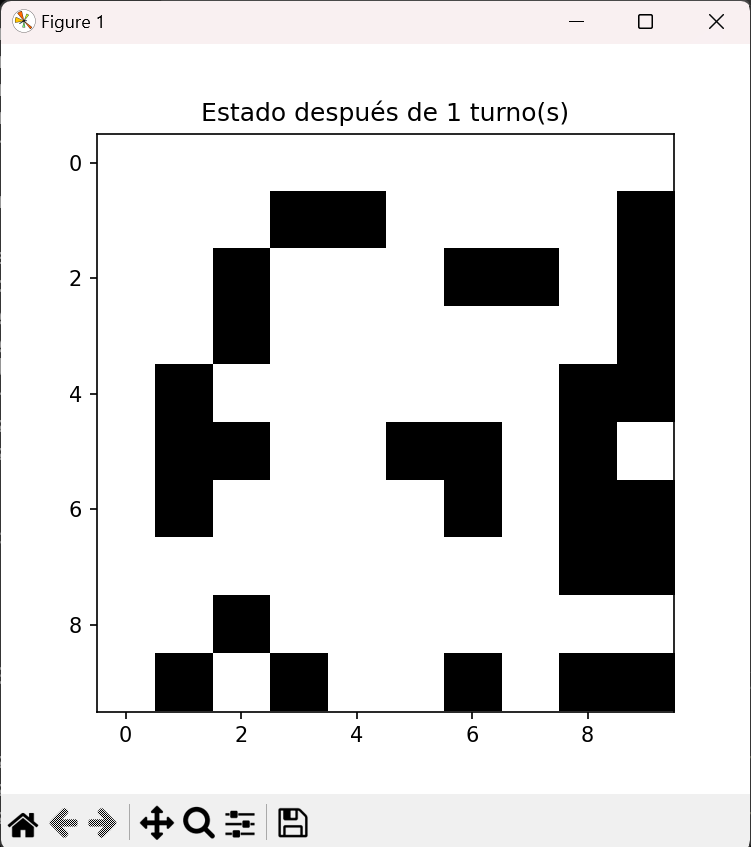
\includegraphics[scale=0.4]{IMA/ejemplosJuegoVida/ejemplo 1.2.png}
        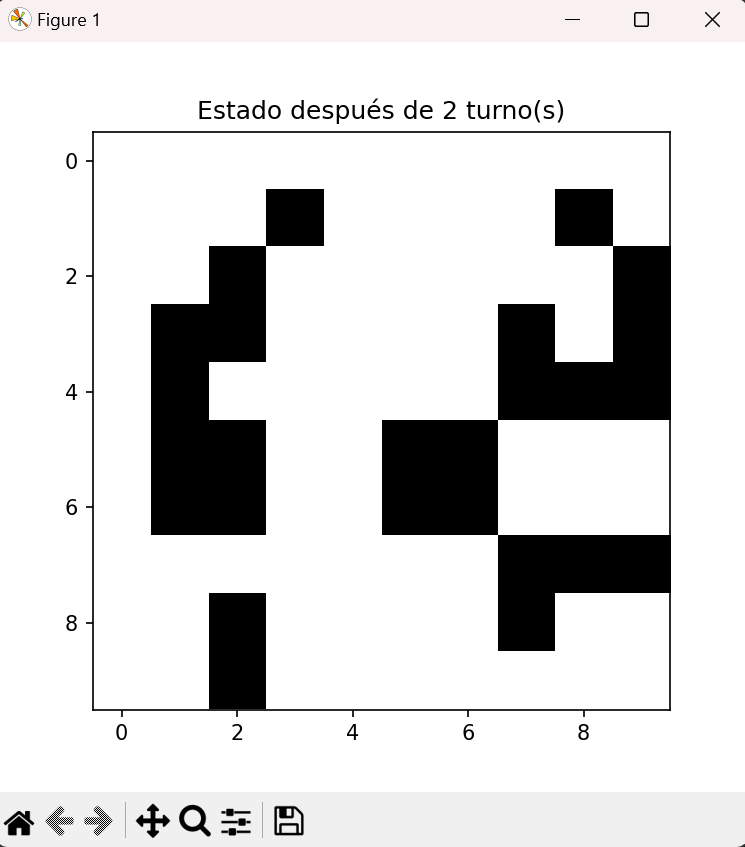
\includegraphics[scale=0.4]{IMA/ejemplosJuegoVida/ejemplo 1.3.png}
        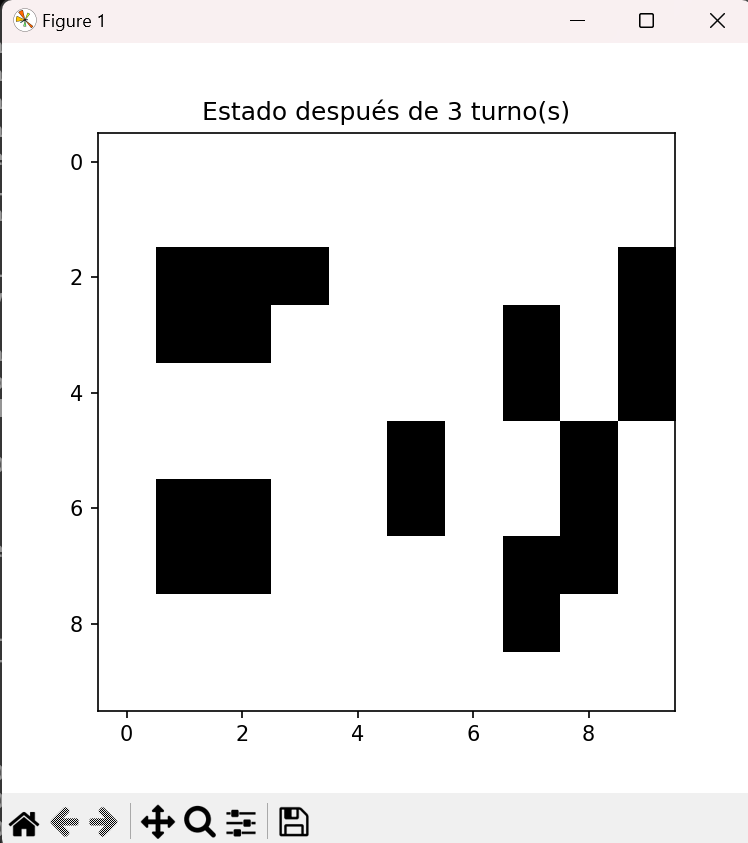
\includegraphics[scale=0.4]{IMA/ejemplosJuegoVida/ejemplo 1.4.png}
        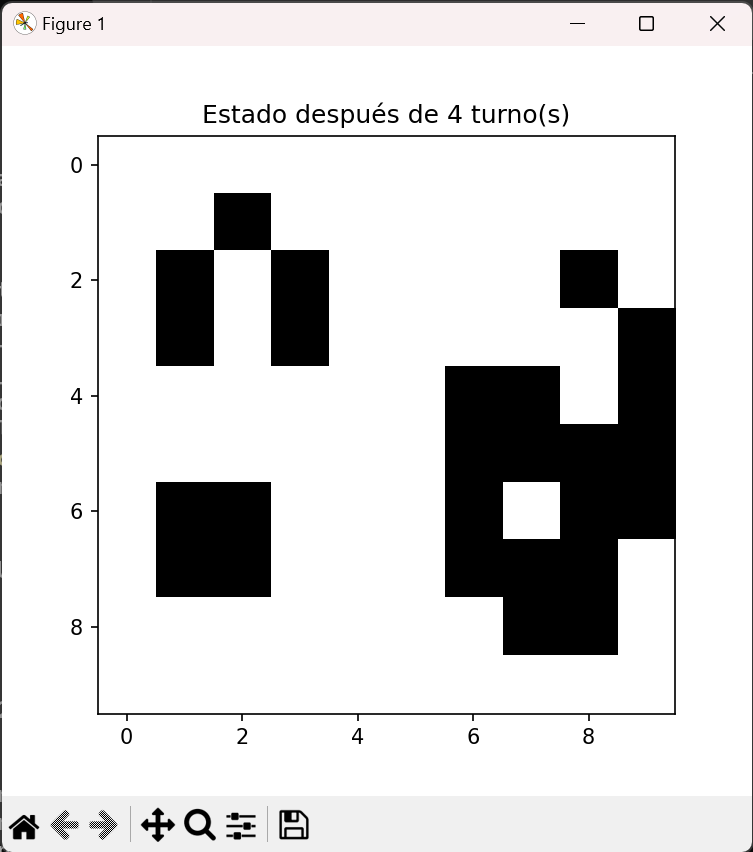
\includegraphics[scale=0.4]{IMA/ejemplosJuegoVida/ejemplo 1.5.png}
        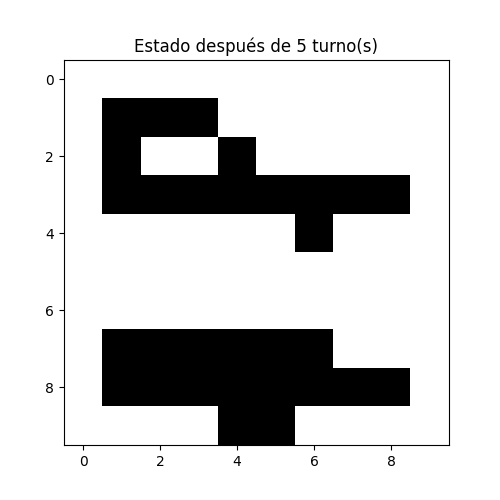
\includegraphics[scale=0.4]{IMA/ejemplosJuegoVida/ejemplo 1.6.png}
    \end{center}

    \item Estado inicial formado

\begin{lstlisting}
# Estado inicial formando un bloque estable
estado_actual = np.array([[0, 0, 0, 0, 0],
                           [0, 0, 1, 0, 0],
                           [0, 0, 1, 0, 0],
                           [0, 0, 1, 0, 0],
                           [0, 0, 0, 0, 0]]) 


# Visualizar el estado inicial
visualizar_estado(estado_actual, "Estado Inicial")

# Bucle para actualizar y visualizar el juego en cada turno
for i in range(num_iteraciones):
    # Aplicar las reglas del Juego de la Vida para obtener el nuevo estado
    estado_actual = aplicar_reglas(estado_actual)
    # Visualizar el estado actual despues de aplicar las reglas
    visualizar_estado(estado_actual, titulo=f"Estado despues de {i + 1} turno(s)")
\end{lstlisting}
    Los estados se muestran de la siguiente forma:
    \begin{center}
        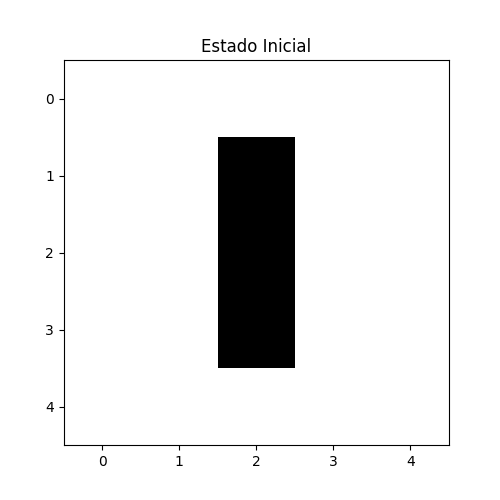
\includegraphics[scale=0.4]{IMA/ejemplosJuegoVida/ejemplo 2.1.png}
        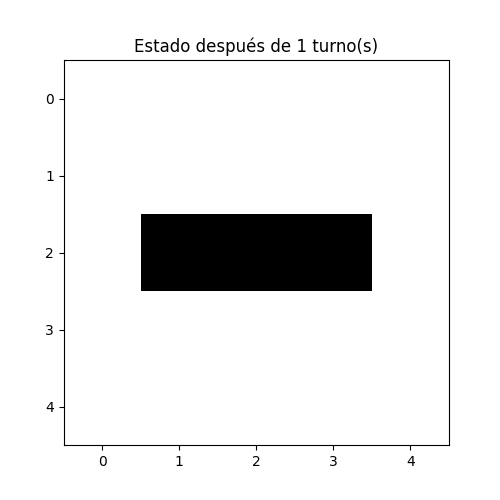
\includegraphics[scale=0.4]{IMA/ejemplosJuegoVida/ejemplo 2.2.png}
        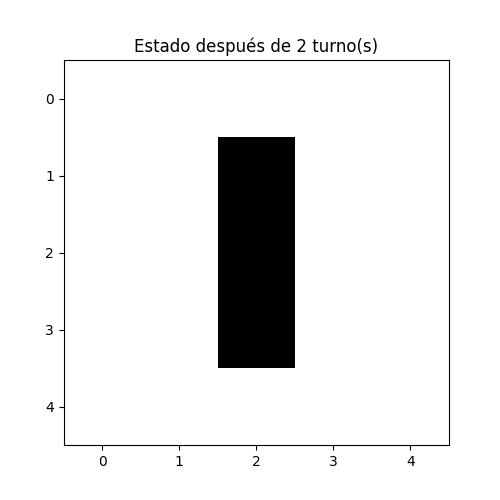
\includegraphics[scale=0.4]{IMA/ejemplosJuegoVida/ejemplo 2.3.png}
        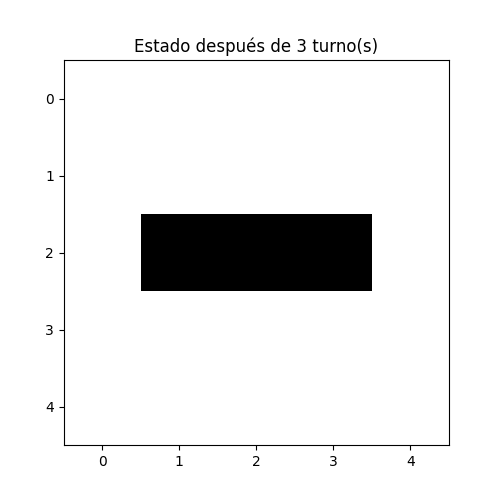
\includegraphics[scale=0.4]{IMA/ejemplosJuegoVida/ejemplo 2.4.png}
        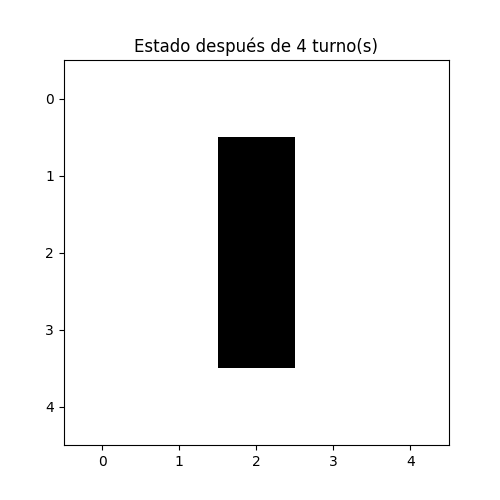
\includegraphics[scale=0.4]{IMA/ejemplosJuegoVida/ejemplo 2.5.png}
        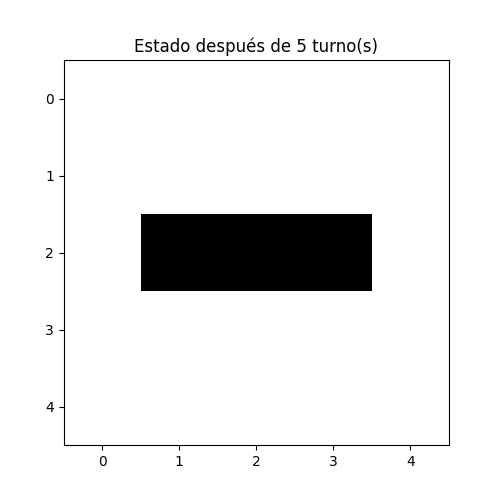
\includegraphics[scale=0.4]{IMA/ejemplosJuegoVida/ejemplo 2.6.png}
    \end{center}    
\end{itemize}


% ----------------------------------------------------------------------------------------\
% ---------------------------------------------------------------------------------------\
\subsection{Juego de la Vida con algoritmo genético}
% ----------------------------------------------------------------------------------------\
% ---------------------------------------------------------------------------------------\

\subsubsection*{Animación}

Usamos la importación de \texttt{import matplotlib} para usar \texttt{matplotlib.use('TkAgg')}
y así poder ejecutar la ventana emergente que muestra la animación del Juego de la vida. 
Mencionamos esto por dos cosas:

\begin{itemize}
    \item Notamos que al ejecutar un archivo \texttt{.py} funciona, al ejecutar un archivo 
    \textit{.ipynb} en nuestro caso dentro de Visual Studio Code funciona la animación pero si
    el código es ejecutado en un archivo de \textbf{colab} truena y aunque quitemos la 
    importación la animación no se ejecuta. 

    \item Se necesito instalar usando el comando (para linux): 
    \texttt{sudo apt install python3-tk}, es para la visualización de gráficos.
\end{itemize}

\subsubsection*{Pruebas}

Nuestro primer caso de salida es cuando hemos agotado la población y no hay 
suficientes para realizar el torneo.
\begin{center}
    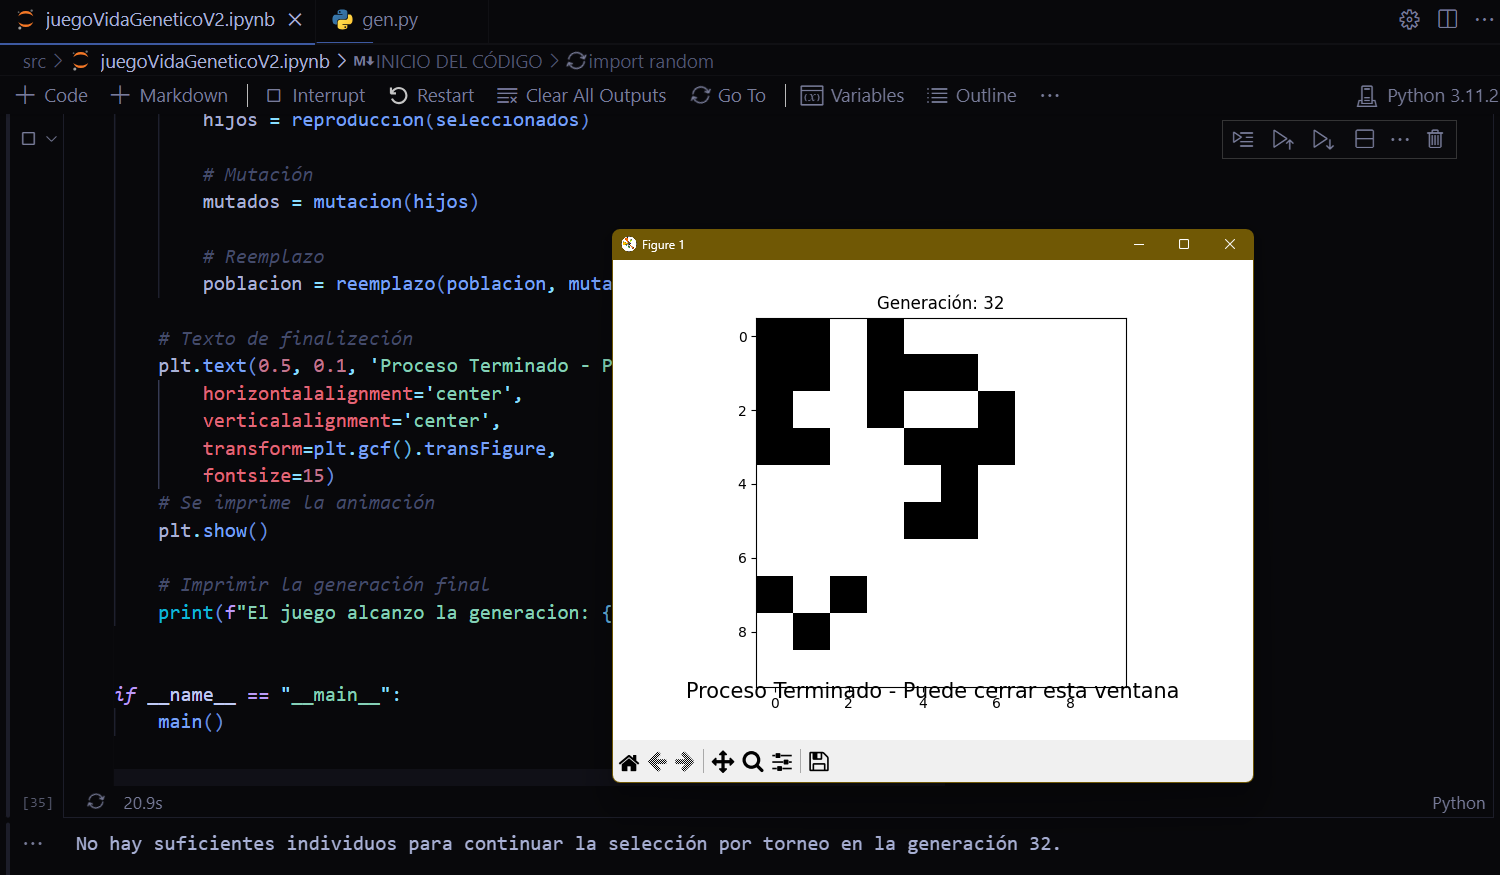
\includegraphics[scale = .4]{IMA/selecTorneo.png}
\end{center}

La segunda salida es cuando la generación no es apta bajo los criterios, por 
lo tanto no hay una nueva generación y tenemos población vacía, entonces 
terminamos.
\begin{center}
    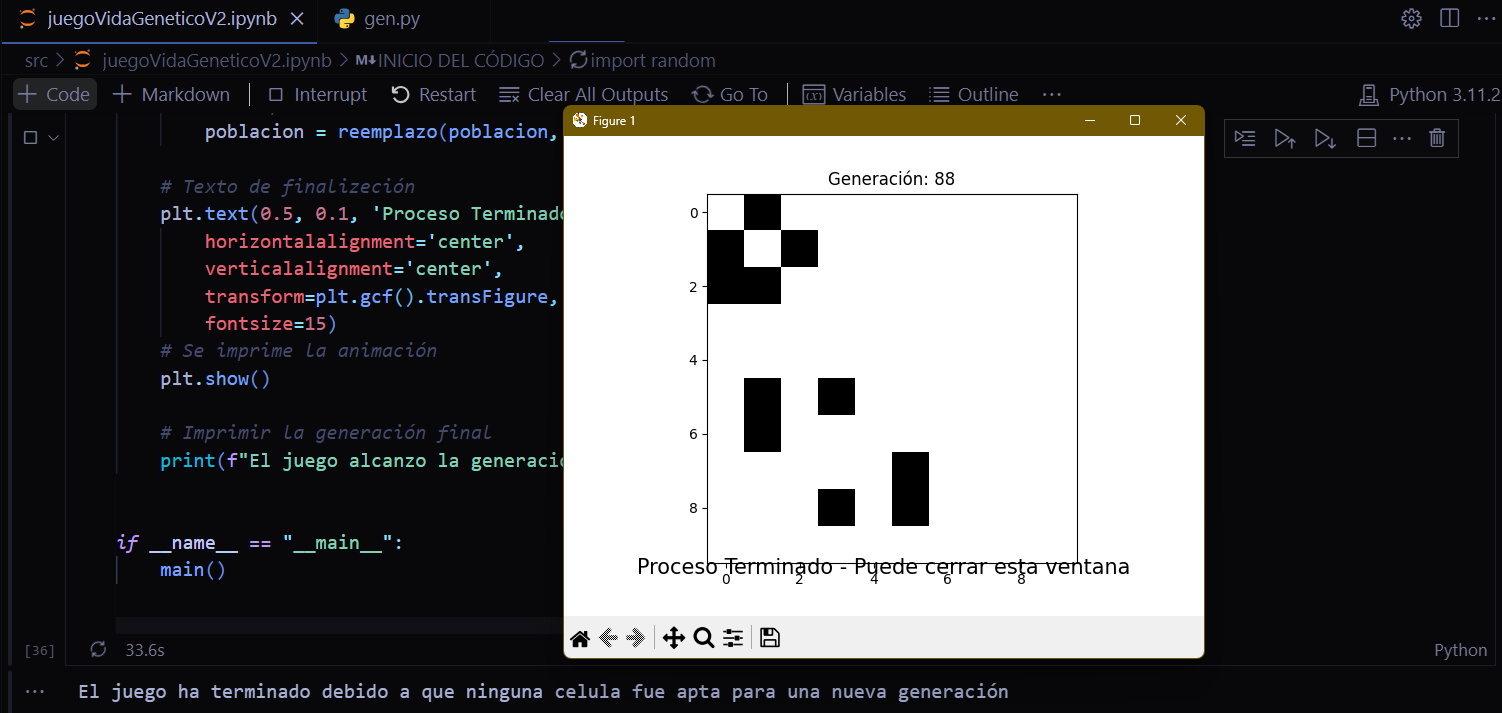
\includegraphics[scale = .4]{IMA/poblacionVacia.png}
\end{center}

Para la tercera salida es el caso especial que condicionamos, donde si nuestro 
porcentaje de células vivas no es mayor después de cierta generación (elegimos
el 70 porciento del total dado) salimos del programa. Esto lo hicimos con la 
finalidad de encontrar células más aptas en menos generaciones. 
\begin{center}
    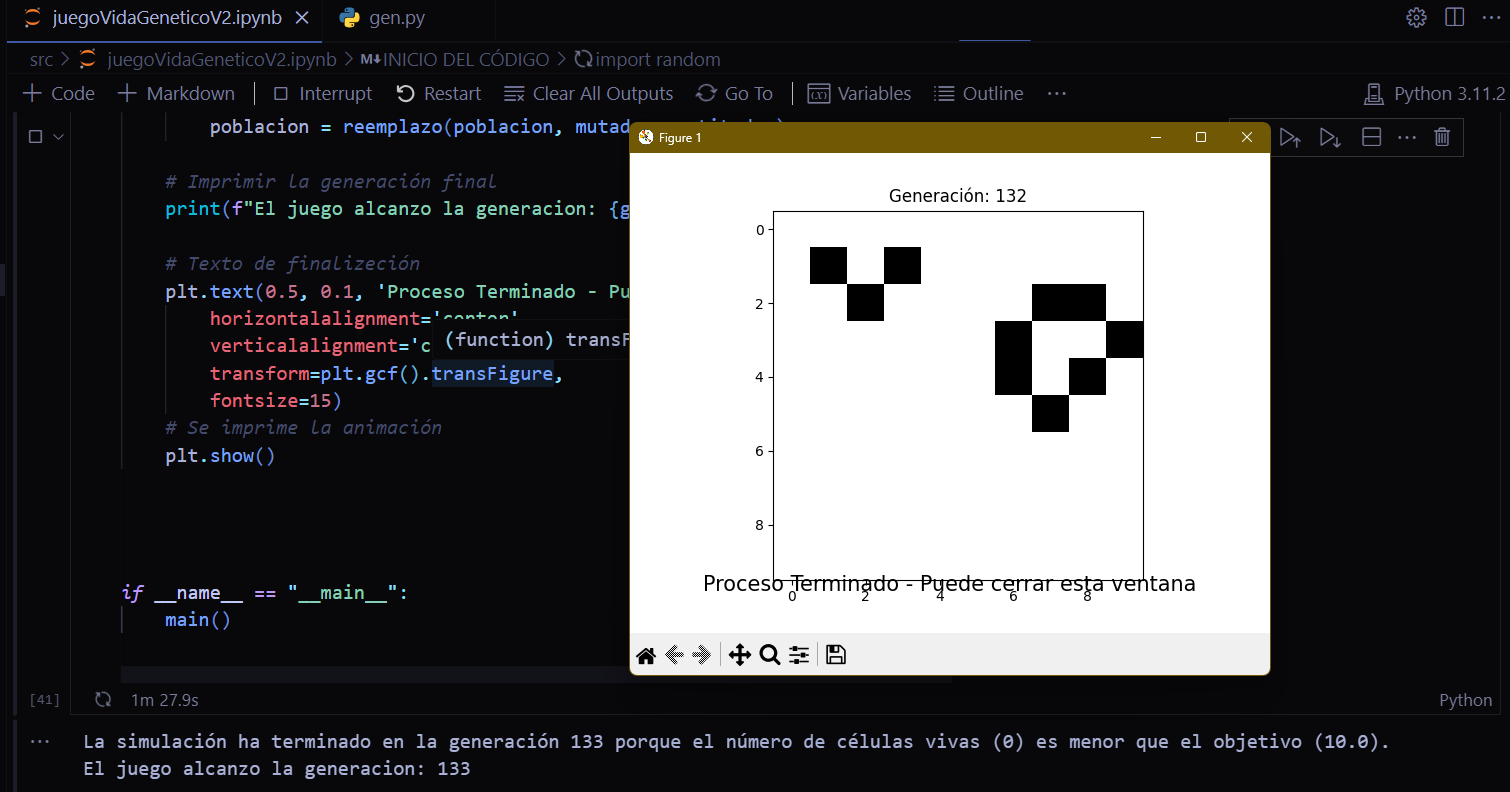
\includegraphics[scale = .4]{IMA/condicionEspecial.png}
\end{center}

Finalmente el caso exitoso donde llegamos al final de las generaciones establecidas. 
\begin{center}
    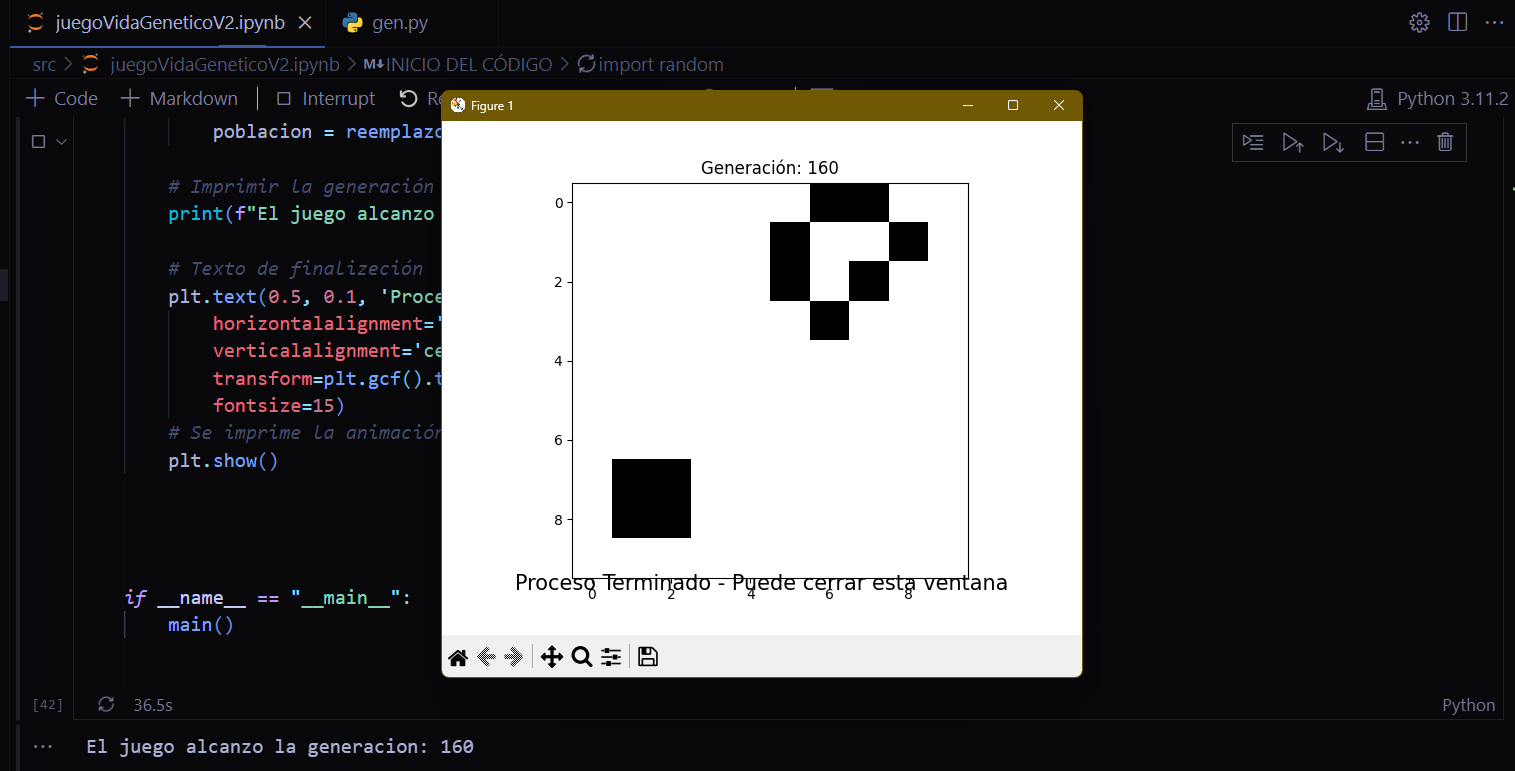
\includegraphics[scale = .4]{IMA/casoExitoso.png}
\end{center}

\subsubsection*{Notas}


Dentro del algoritmo se definieron constantes con las que hemos jugado a lo largo de 
la creación del algoritmo, comprobamos la importancia de la función de aptitud para
llegar a nuestro objetivo a demás de ver como las mutaciones en este caso particular 
pueden ser buenas y malas. 

Las constantes son:
\begin{itemize}
    \item \texttt{TABLERO} Se define un tablero cuadrado y podemos jugar con el tamaño
    de sus lados para que a medida que células más aptas crezcan podamos observar patrones
    generados, cosa que no es tan visual con tableos pequeños.

    \item \texttt{POBLACION INICIAL} Comprobamos que para nuestra solución entre menos 
    población habrá menos oportunidades de éxito, una posible mejora para tratar eso sería 
    modificar nuestra función de torneo. 

    \item \texttt{GENERACIONES} Son la medida para saber que tanto funciona nuestra función 
    de aptitud junto con el número de células vivas objetivo. 

    \item \texttt{OBJETIVO CELULAS VIVAS} El porcentaje que deseamos este cubierto de células 
    vivas dentro del tablero.

    \item \texttt{C} Es la constante que nos ayuda para la formula de las astronaves.   
\end{itemize}

% ----------------------------------------------------------------------------------------\
% ---------------------------------------------------------------------------------------\
% --------------------------------------------------------------------------------------\
\section{Reflexión final}
% ----------------------------------------------------------------------------------------\
% ---------------------------------------------------------------------------------------\
% --------------------------------------------------------------------------------------\

Para el juego de la vida, dentro de sus reglas originales hemos visto que depende mucho la 
primera itereción en como afectara todo el desarrollo del juego habrá ocacionesn en las que 
(tambien dependiendo del tamaño del tablero) se verá la velocidad como va creciendo y 
creciendo la población o como tambien se va moviendo por el tablero, en ocasiones será muy 
bajo y en otros mul alto el contenido de las celulas vivas. \\


En nuestra modificación de las raglas queriamos llegar a tener un tablero mucho más poblado 
despues de ciertas generaciones, esto lo lograriamos por medio de la función de aptitud, esto 
combinado con la aplicación de un algoritmo genetico nos permitio observar grandes cambios 
respecto a como se ejecuta simplemente las reglas. \\

Es decir, cuando solo se aplican las reglas dependemos dependemos de que tan buena sea la forma 
aleatoria inicial, pero con un algorimo genetico, vemos como va aprendido de nuestra función de 
aptitud. Cada iteración es diferente y lo comprobamos por nuestras cuatro clausulas de salida.\\

La resolución del juego dependera de las reglas y el objetivo que se dese alcanzar, pero sin 
duda aplicar un algorimo genetico ayudará a guiar la solución a travez de las generaciónes y 
de que buena sea la estructura de la función de aptitud, además del factor mutación, vimos 
en varias iteraciónes que el algorimo llegaba a un punto de ciclos y con la mutación salia. 



% Después de las simulaciones, analizar cómo la evolución de los cromosomas afectó el 
% desarrollo del Juego de la Vida, identificando patrones o estrategias exitosas.

% Redactar un breve informe que reflexione sobre el aprendizaje obtenido, las estrategias 
% que resultaron ser más efectivas y cómo los principios de los algoritmos genéticos 
% podrían aplicarse a otros problemas de optimización o simulación.